\chapter{Data Mining in Nearby Galaxies}
%----------------------------------------------------------------------------------------
%----------------------------------------------------------------------------------------
%----------------------------------------------------------------------------------------
%Intro
%----------------------------------------------------------------------------------------
%----------------------------------------------------------------------------------------
%----------------------------------------------------------------------------------------
\section{Introduction} %%( I am not really happy with this introduction but it is the best I can have for now:/ )
%General information about galaxies %(Maybe it is too generic?!!)
Inside each galaxy, there are millions of stars and large amount of dust and gas, which all affect on each others' formation, evolution and extinction.
Galaxies are an active and complicated systems, that are constantly changing.
There are extensive amount of studies about correlations between galaxies' emission and their physical properties, both observationally and theoretically %(Some references here). 
These studies expands our knowledge of the underlying processes in formation and evolution of galaxies every day, but the details of how these process work are still undetermined.

% Nearby galaxies and their importance 
Nearby galaxies play an important role in learning about galaxies' formation and evolution.
These galaxies are close enough to be able to observe various regions inside them in details.
As a result, many studies are devoted to find relations between physical properties of the galaxies in both spatially resolved regions and galaxies as a whole%(Some more references here)
, and many others use these results in analyzing data from high-redshift galaxies. %(Some more references here)
The amount of data that is acquired from nearby galaxies is increasing daily.
Advances in technology helps to both observe and store enormous amount of data from sky.%The sky?! 
Telescopes and surveys gather data from nearby galaxies in variuse wavelengths and from these data we can measure physical properties of galaxies (e.g. stellar mass, star formation rate (SFR), dust mass, gas mass)~\citep[e.g.][]{Calzetti07,Dale09,Eskew12}.

% A little bit about M31 and previous studies in M31.
The Andromeda galaxy (M31), with a distance of $\sim$0.78~Mpc~\citep{McConnachie05}, is the closest spiral galaxy to the Milky Way.
Images of this galaxy provide us a detail view of inside of a spiral galaxy from distance.
M31 data was a target of many telescopes (e.g. {\it Hubble} \citep{Dalcanton12}, \Spitzer\citep{Wener04}, \Herschel\citep{Pilbratt10} space telescopes) and was a subject of many more studies \citep[e.g.][and references therein]{Barmby06, Gordon06, Azimlu11, Sanders12, Dim15, Rahmani16}. 

\cite{Barmby06} used data from Spitzer Infrared Array Camera \citep[IRAC;][]{Fazio04} to show evidence of Polycyclic Aromatic Hydrocarbons (PAH)s in interstellar medium (ISM) of M31.
Using the mid-IR data from Multiband Imaging Photometer for Spitzer (MIPS), \cite{Gordon06} studied the morphology of the dust in M31.
\cite{Azimlu11} and \cite{Sanders12} catalogued and studied H {\sc II} regions of M31.
\cite{Draine14, Mattsson14, Viaene14, Smith12} and~\cite{Fritz12} used \Herschel data to study dust in the ISM of the galaxy.
Properties of the current stars in the galaxy were studied by~\cite{Tamm12} and~\cite{Massey07}. %%%And some from PHAT survey
\cite{Rahmani16, Ford13} and \cite{Tabatabaei10} measured the SFR in M31 in order to study star formation laws, and \cite{Dim15} and \cite{Kapala15} used spectroscopic data of the galaxy to study PAHs and other line emissions in the ISM.

Although all these studies measured some properties of M31, or answered specific scientific questions about this galaxy, we still do not have a complete picture of undergoing processes in the galaxy.
The amount of the observed data and measured quantities of M31 makes this galaxy a suitable target for a knowledge discovery and data mining study.
Knowledge discovery and data mining methods are designed to extract hidden information from data and are tested in many astronomical studies.
However, to the best of our knowledge, this study is the first study that uses a data mining method on data from nearby galaxies. %%% ehh

% data mining and clustering in general; when we have so many data and we want to map them
\cite{Ball10} wrote an extensive review of data mining and machine learning, and their usages in astronomy.
A data mining algorithm learns about data from sets of trainings, which can be supervised or unsupervised.
The supervised trainings refer to methods, that use examples of the desired output to learn about input data and are valuable tools to classify data with known target values.
On the contrary, the unsupervised methods train without any prior knowledge of output results. 
They solely work based on the underlying structure of input data.   
The unsupervised methods are very useful tools in knowledge discovery studies on input data, which we do not have any insight of them (or when we want to make sure that we did not miss any valuable information in our previous studies). %%% ehh to after or part.

%SOM
One the most tested methods of data mining in astronomy is the artificial neural networks (ANNs)~\citep[e.g.][and references therein]{Hossein12, Hossein14,Hossein16,Ellison16a}.
ANNs are designed to work in the same way that the neurons work in a human mind.
They are networks of interconnected neurons (nodes), which all of the connections are weighted.
These networks are used to study about nonlinear and complex relations between input and output data.
%These relations can be applied to the new sets of data with similar feature

One of the most well-known unsupervised neural network in astronomy is a Kohonen self-organizing map (also called self-organizing map, or SOM).
SOMs map and visualize a complex and nonlinear high dimension data~\citep{Kohonen82} and show simple geometrical relationships in non-linear high dimensional data~\citep{Kohonen98}.
The result of a SOM is a 1D or 2D network of neurons, which shows the positions of clusters and their relative distance.
Since 1990s, many studies utilized SOMs for object classification and clustering (e.g. classifying quasars' spectra, star/galaxy classifications, gamma-ray bursts clustering and classification of light curves), and photometric redshift estimations~\citep[e.g.][]{Odewahn92, Hernandez94, Murtagh95, Maehoenen95,Scaringi09,Geach12,Fustes13,Meusinger16,Rahmani16b} %%% Why I cannot add submitted in front of the high-z paper

% other Unsupervised methods
The purpose of this project is to have a new insight into nearby galaxies using M31 data with focusing on relations between PAHs and other properties of the galaxy.
To fulfill this purpose, an unsupervised data mining method is the most suitable choice. %%eh  
K-means algorithm, SOMs, and hierarchical clustering are main unsupervised methods that are used in astronomical studies~\citep[e.g.][]{DAbrusco12, Aycha16}. %%add one or two more

For both K-means and SOM algorithms, the user must define the number of clusters, and the algorithms decide how to separate the data into desired number of the clusters.
In the hierarchical clustering method, the user must define dissimilarity between the groups, and the algorithm combines (or divides) existing groups based on their dissimilarity and creates a hierarchical structure. 
Comparing SOMs, K-means and hierarchical clustering shows that in some cases hierarchical clustering method miss-classifies the data~\citep[][and references therein]{Mangiameli96}.
We chose SOM method over K-means due to the fact that SOMs not only clusters data, but also shows similarity and dissimilarity between each cluster.
Therefore, we can cluster our sample data and study the underlying structure of data, simultaneously.

%this project 1 M31 and its extensive data we do not have any SOM in nearby galaxies
In this project we apply SOM algorithm on M31 data, and trained 1D and 2D networks.
Using smaller size networks we study the properties of the clusters and investigate relations between PAHs features with other features in M31.
We create 2D SOMs from subsets of data as well as all available data, which helps us to understand the effect of each input in the position of the clusters in the SOM, which leads to prediction of the unmeasured quantities in a galaxy.
Assuming that all the spiral nearby galaxies have similar properties, we apply 2D trained networks on data from the Pinwheel Galaxy (M101), which is another spiral nearby galaxy. 
If our hypothesis is correct, we should be able to see that regions in M31 and M101 with the same positions in the SOM have the same properties.

In Section $\S$~\ref{Sec: data_SOMN}, we present the sample data from M31 and M101, that we use in this study. 
We describe the SOM method in Section $\S$~\ref{sec: method}. 
The results of the 1D SOM networks and studying PAHs in M31 is presented in Section $\S$~\ref{Sec: 1d_cluster}.
In Section $\S$~\ref{sec: 2d_cluster}, we present the result of 2D SOM networks and how we use them to extract information about other galaxies.
In Section $\S$~\ref{sec: summary}, we summarize our results and discuss potential future work in this subject.



%----------------------------------------------------------------------------------------
%----------------------------------------------------------------------------------------
%----------------------------------------------------------------------------------------
%DATA
%----------------------------------------------------------------------------------------
%----------------------------------------------------------------------------------------
%----------------------------------------------------------------------------------------

\section{Sample of study}
\label{Sec: data_SOMN}

We gathered data from 10 regions in M31 (Fig.~\ref{fig: regions in m31}) and 8 regions in M101 (Fig.~\ref{fig: regions in m101}) as inputs for SOMs.
We chose those specific regions due to availability of the PAHs data for them.
Besides PAHs data, for each galaxy, we chose spectroscopy and photometry data as well as their derived properties, such as SFR, stellar mass, dust luminosity (L$_{\rm dust}$) and mass, metallicity, and gas mass.
Table~\ref{tab: data} shows the full list of the data and their unit for both M31 and M101.
We divided each values by the area of their region (in arcsec$^2$), to remove the distance factor from the data compare values of quantities in both galaxies.
Since the resolution of the data varies from less than 1$\arcsec$ to $60\arcsec \times 90 \arcsec$, any attempt to match the resolutions causes loosing all the information in some of the input data (e.g. the spectroscopic data).
On the other hand, in this project we used flux (or value of the quantities) per area as inputs of SOMs, which the convolution methods conserve it~\citep{Aniano12}.
Therefore, we did not perform any resolution matching in this paper and used data in their original resolutions.


\import{../image_paper3/text_files/tables/}{tab_data.tex}


  \begin{figure*}
    \subfloat[MIPS 24~$\mu$m image of M31 from~\cite{Gordon06}, with position of 10 regions \label{fig: regions in m31}]{
      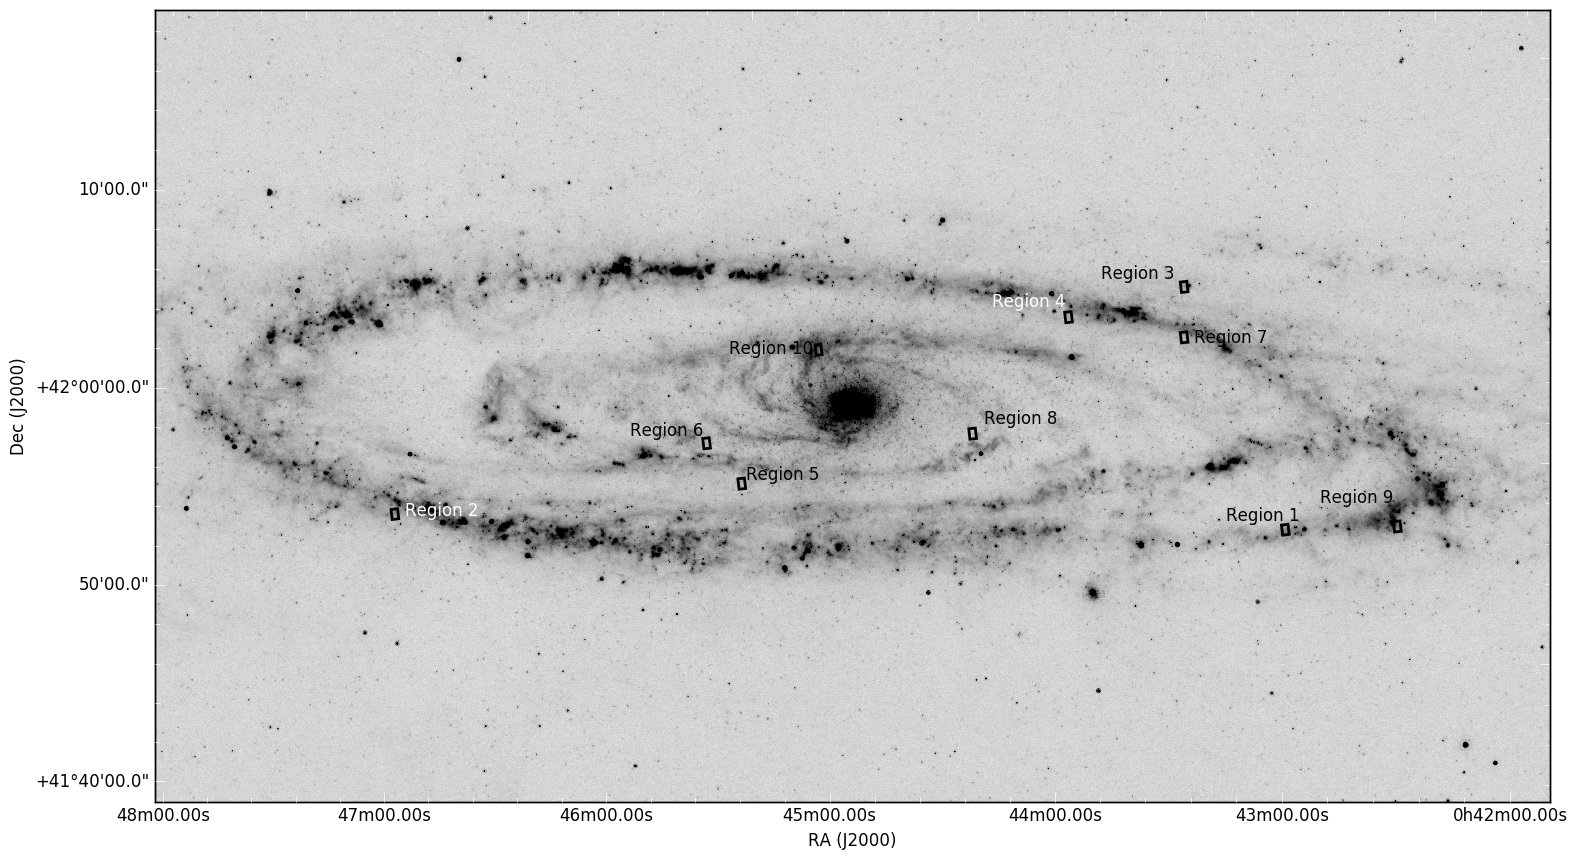
\includegraphics[width=\textwidth]{../image_paper3/images0.0/M31/M31.png}
    }
    \hfill
    \subfloat[IRAC 3.6~$\mu$m image of M101~\cite{Dale09}, with position of 8 regions.\label{fig: regions in m101}]{
      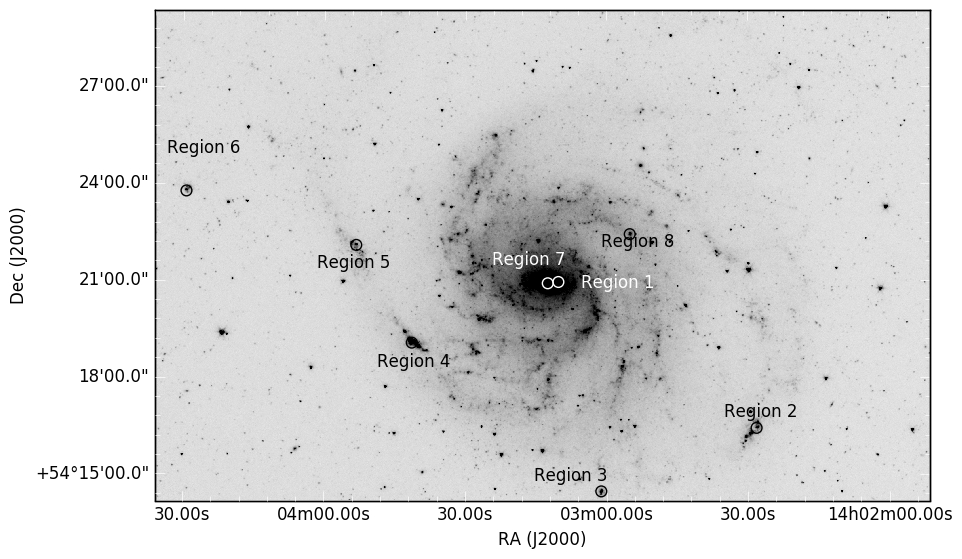
\includegraphics[width=\textwidth]{../image_paper3/images0.01/M101/M101.png}}
    \caption{Position of regions that the input data for SOM that obtained from there in M31 (up) and M101 (down).}
    \label{fig:dummy}
  \end{figure*}
  
%M31 data 
%%%%% Sahar: More detail, right?
    \subsection{M31 data}
     \label{Sec: data_M31_SOMN} 
     
     The 10 regions in M31 were chosen due to availability of the PAH data for them. 
     \cite{Dim15} studied PAH for those regions using {\it Spitzer}/Infrared Spectrograph~\citep[IRS,][]{Houck04b} observations. 
     They used {\sc PAHFIT IDL} tool~\citep{Smith07b} and measured fluxes and equivalent widths of PAH features as well as atomic line features.
     %For spectroscopy part of our sample, we utilized their measured fluxes for PAH lines. 
     \cite{Dim15} also measured metallicity and of radiation hardness index (RHI) for these 10 regions.
     We used the measured fluxes for PAHs featured, metallicity and RHI of each region as an input for SOMs.
     
     We used \GALEX FUV and NUV channels~\citep{Martin05}, \halpha, [\sii] narrow badn and [\oiii] narrow band~\citep{Massey07}, IRAC channels 1 to 4~\citep{Barmby06}, MIPS24 and 70~$\mu$m~\citep{Gordon06}, PACS100 and 160~$\mu$m and SPIRE250, 350, and 500~$\mu$m~\citep{Fritz12} emission for photometry part of the sample.
     We changed units of all fluxes to Wm$^{-2}$ to be the same unit as PAHs fluxes.
     $^{12}$CO (J:$1\rightarrow0$) line~\citep{Nieten06} and the atomic gas (H\,{\sc I}) 21~cm emission from~\cite{Chemin09} were added to the input data. 
     For derived values, we utilized SFR(FUV + 24$\mu$m), stellar mass, mass of molecular clouds, mass of atomic gas (H\,{\sc I}), total gas mass, and total infrared (TIR) luminosity (L$_{\rm TIR}$) data from \cite{Rahmani16}, and L$_{\rm dust}$ and mass data from \cite{Draine14}.
     
    \subsection{M101 data}
    \label{Sec: data_M101_SOMN} 
     For M101 galaxy, we used PAH fluxes which had been measured using {\sc PAHFIT IDL} tool and reported in \cite{Gordon08}.
     We also added their measurement of metallicity and RHI for these regions to our sample.
     We used data available on NED~\footnote{The NASA/IPAC Extragalactic Database (NED) is operated by the Jet Propulsion Laboratory, California Institute of Technology, under contract with the National Aeronautics and Space Administration.} website to gather our photometry data of M101. 
     We chose data from \GALEX FUV and NUV channels~\citep{depaz07}, IRAC channels 1 to 4, MIPS~24 and 70~$\mu$m~\cite{Dale09}, and  PACS~100 and 160~$\mu$m and SPIRE250, 350, and 500~$\mu$m emission from~\cite{Kennicutt11}.
     The Same as M31 data, we used $^{12}$CO (J:$1\rightarrow0$) line~\citep{Helfer03} and the atomic gas (H\,{\sc I}) 21~cm emission from \cite{Walter08} data.
     SFR(FUV + 24$\mu$m), stellar and total gas mass map were calculated using the same methods that M31 data were derived in \cite{Rahmani16}.
     
      Some of the correlations between some wavelengths and properties of galaxies are well-known.
     For example, \citep{Rahmani16} used IRAC1 band emission to calculate the stellar mass, or FUV, NUV and MIPS24 emission to measure the SFR values. 
     To make sure that we wouldn't use some of the observed data as an input data in various forms, we removed all the observed data, that were used to calculate these properties from the input sample.
     We used these sample as the main input for creating SOMs.
     Fig.~\ref{fig: cor_all} shows Pearson correlation coefficients with a confidence level of $95\%$ for the input data.

     
      \begin{figure}
                \centering
                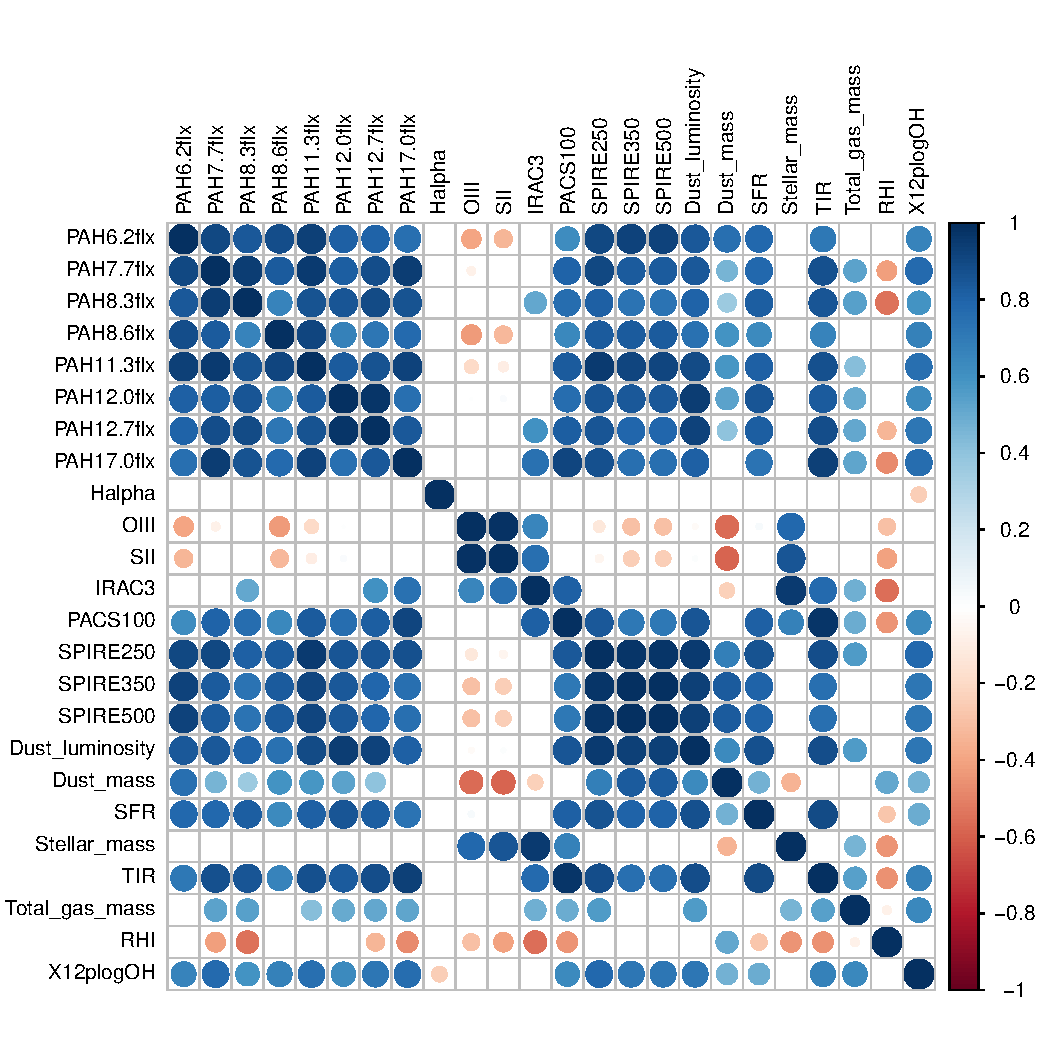
\includegraphics[width=\textwidth]{../image_paper3/images0.01/cor_plots/M31_all_derived_ones_core_plot_for_paper.pdf}
            \caption{Pearson correlation coefficients with a confidence level of 95$\%$ for all the in the subset 0. The colours show the Pearson correlation coefficients where 1 means highly correlated and -1 is highly anti-correlated quantities. The non-significant correlations were left empty.}
            \label{fig: cor_all}
        \end{figure}
 
  
%----------------------------------------------------------------------------------------
%----------------------------------------------------------------------------------------
%----------------------------------------------------------------------------------------
%Method
%----------------------------------------------------------------------------------------
%----------------------------------------------------------------------------------------
%----------------------------------------------------------------------------------------

\section{METHOD}
\label{sec: method}
 \subsection{Self Organizing Maps}
 \label{sec: som}
 The SOM is a clustering method which reduces the dimension of data to lower dimensions, while preserving topological features of the original data~\citep{Kohonen98}. 
 The results of the SOM are shown with a map of neurons.
 Each neuron has a fixed position in the map, and may contain one or more samples from input data, \boldit{V} $\in \Re^n$.
 A weight vector,~\boldit{W} $\in \Re^n$, with the same dimension as the input data is associated with each node and will be varied during the training process.
 The process of creating SOM, happens over series of $N$ iterations.
 In each iteration, the algorithm calculates the euclidean distance for each node j as  $D_j^2= \sum_{i=0}^{i=n} (V_i - W_i)^2$, and finds a neuron with ``$D_{j_{min}}$". 
 This neuron is the winner node and is calling Best Matching Unit (BMU). 
 The weight vectors in the neighbourhood of BMU will change according to the Kohonen learning rule (equation~\ref{equ: weight adj}). 
  \begin{equation}
            \label{equ: weight adj}
            w(t+1)=w(t)+L(t) \times R(t) \times(v(t)-w(t))
 \end{equation}
where $L(t) = L_0 e^{(-t/\tau)}$ is the learning factor, which prevents the divergence of the SOM and $R(t)=\exp(-\frac{D_j^2}{2r^t_{BMU}})$ is the influence rate, which determines how the weight of each node will change.
Values for number of neurons, L(t) and R(t) are arbitrary. 
~\cite{Geach12} and \cite{Rahmani16b} demonstrate the algorithm of the SOM in more details.


     In order to create SOM, we used {\sc MATLAB} neural network toolbox~\citep[NNT,][]{matlabtolbox}.
     An SOM in {\sc NNT} can be created by {\sc newsom} library which works in two phases; ``ordering phase" and ``tuning phase" . 
     Phase one is the ``ordering phase". 
     This phase starts with maximum neighbourhood distance, and initial high learning factor usually 0.9 which is provided by user. 
     The ordering phase continues for requested number of iterations and it continues till the learning factor reduces to tuning phase leaning factor and the neighbourhood distance reaches to the number set by the user.
     
     The second phase is the ``tuning phase".
     In this phase the neighbourhood distance is at its minimum, but learning factor decreases very slowly.
     This minimum neighbourhood distance and slowly decreasing the leaning factor helps to fine tune the topology results and causes the more stable SOM. 
     The number of iterations in this tuning phase most be much more than the number iterations in ordering phase, to allow the tuning happens slowly. 
     We chose number of epochs the tuning phase be 3 times more than number of epochs in the ordering phase.
     
     To present our results, we use {\sc nnt}'s built-in plotting tool.
     Specifically, we combine two of the plots in this tool: a hits map, which shows the number of times each neuron has became the winner (hits), and a distance map, which shows the distance between weight vectors of those neurons.
     In the maps, the purple hexagonal shapes shows the neurons. 
     The distances are shown by the grey cycle colours: the darker the colour, the larger the distance between neurons.
     Neurons with zero hits are left empty.
     In Section~\ref{sec: mock_sample} we used {\sc newsom} to create SOMs from a mock sample to illustrate how this method works and how we can interpret the results.

     One feature of the SOM method is that there is no rule and restriction on number of clusters.
     Users must decide the size of networks based on their data set and their usages of the results .
     There has been few attempts to find a rule for restricting the number of neurons based on the input sample \citep[e.g.][]{Vesanto05}, but none of them are certain. 
     We varied size of SOMs from $1\times2$ to $50\times50$ to choose the most suitable size for our maps, and found that based on the size of our sample, the 2D SOMs to be 10$\times$10. 
     We create the final SOMs with initial values for number of iterations in ordering phase, ordering phase learning factor, tuning phase learning factor, and tuning phase neighbourhood distance of 500, 0.9, 0.02, and 1, respectively. 
     %Also for each grid we created different SOM with different, learning factors, neighbourhood distances, and iteration numbers to find the optimize result for our sample.
     %Based on our data we created our final SOMs with following initial values: number of iteration in ordering phase = 1000; ordering phase learning factor = 0.9; tuning phase learning factor= 0.02; and tuning phase neighbourhood distance to be 1.
     %All the other parameters are default values in {\sc newsom} library and cannot be changed by the users. 
     
    
\subsection{Mock sample}
\label{sec: mock_sample}
 
         \begin{figure}
                \centering
                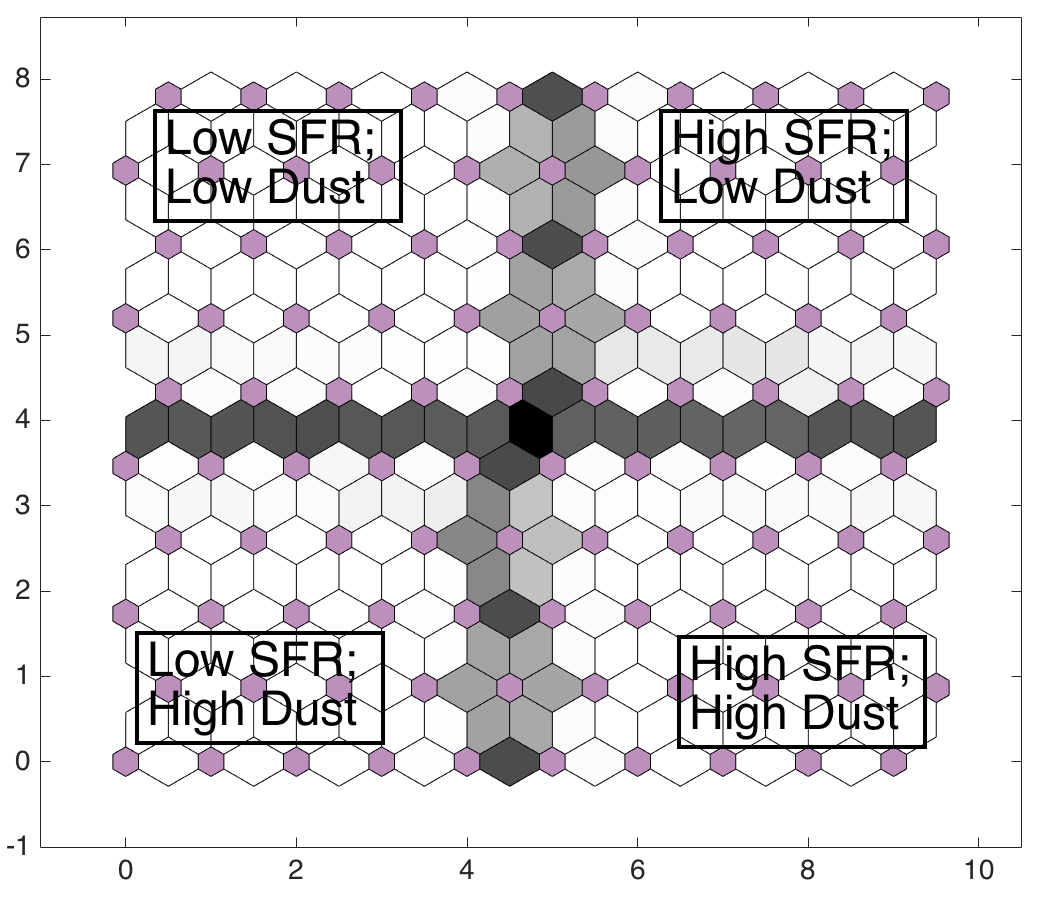
\includegraphics[width=0.5\textwidth]{../image_paper3/images0.01/mock_sample.png}
            \caption{SOM of the mock sample. The axes show the position of the neurons. Hexagonal shapes represent the neurons. The grey cycle colours show the differences between weight of each neuron where white is the minimum differences and black has the maximum one.}
            \label{fig: sample}
        \end{figure}
 
To show how self-organizing maps work, we created a mock sample, which contains a few regions.
We gave two information to each sample; amount of dust and the SFR.
 Therefore, we have a simple input data with low dimension; each entry only can get either 0 or 1 as high or low SFR, and 0 or 0.5 to show high or low amount of dust for the mock regions.
 We generated an SOM with the size of $10 \times 10$ from the sample, using the method that described in Sec.~\ref{sec: som}.
 Fig. ~\ref{fig: sample} shows the SOM of the mock sample. 
 The axes show the position of the neurons in a $10 \times 10$ network and the hexagonal shapes are the neurons.
 
Using this method, as expected, we are able to divide the mock sample into 4 distinct groups: regions with high SFR and high amount of dust, regions with low SFR and high amount of dust, regions with high SFR and low amount of dust, and regions low SFR and low amount of dust. 
The plot in the Fig.~\ref{fig: sample}, clearly shows these divisions.
In that plot, the upper part belongs to regions with low amount of dust, while the lower part belongs to the high amount of dust.
The left part of the plot, is where regions with low SFR belong to and the right side is for high SFR regions.
Grey to black colours show the border between regions.
This network is considered as a trained network, and can used to cluster any new data set with similar entries.

Having two regions with exactly the same values in all their quantities in the real world is almost impossible. 
Therefore, one can find a network with high amount of the neurons, which separates the input data completely, and clusters them into separate groups.
However, if the input data has high similarity, the number of neurons must be much higher than the number of input samples to be able to separate the groups from each other. 
Therefore, it is up to the user to decide the similarity or dissimilarity between the input data based on the number of neurons. 

%----------------------------------------------------------------------------------------
%----------------------------------------------------------------------------------------
%----------------------------------------------------------------------------------------
%Result Part 1: 1D SOMs
%----------------------------------------------------------------------------------------
%----------------------------------------------------------------------------------------
%----------------------------------------------------------------------------------------
\section{One dimensional Self-organizing maps}
    \label{Sec: 1d_cluster}
%Why 1D maps are useful
    The purpose of the exploring M31 data with 1D maps is to monitor the general behaviour of data. 
    1D SOMs can have from the minimum number of clusters, $1\times2$, to the highest number of cluster possible.
    In a small sample like ours, smaller grid SOMs are very useful to find correlations that cannot be found without the clustering the data.
    On the other hand, higher grid 1D SOMs are a helpful tool to get quick insight into data.
%    In the following section, we are going to show how we used 1D SOMs to extract information from available data in M31.
%Clustering
 %   \subsection{Clustering M31 data}

        In order to monitor how the data behaves, we created SOMs with two to fourteen neurons (Fig.~\ref{fig: M31_nets_1d}).
        The $1\times2$ network (Fig.~\ref{fig: M31_net_1by2}) shows how the M31 data can be divided into two broad categories.
        While the $1\times14$ network (Fig.~\ref{fig: M31_net_1by14}) is the first network that all the regions in M31 are completely separated.
        Since in the higher network sizes, regions have more space to be separated based on their differences, we can see that from $1\times2$ to $1\times14$ network the M31 regions separated from each other increasingly, until they are completely separated. 
        
        In Fig.~\ref{fig: M31_net_1by2}, it is clear that by forcing the regions in the M31 to be divided into two groups, regions 1, 2, 9 and 10 occupy one neuron and the other regions occupy the other one.
        The medium grey colour between two neurons indicates that there are some similarity between two groups, but they are not very similar. 
        By increasing the size of the neurones to three, in Fig.~\ref{fig: M31_net_1by3}, we can see that the region 2 separates itself from the other regions and occupies the middle neuron.
        The white colour between two left neurons suggests that regions, which occupy these neurons are very similar to each other, while the black colour between two right neurons expresses otherwise.
        
        %%%Talking about four right regions
        \cite{Dim15} showed that the regions 1, 2, 9, and 10 have higher PAHs flux intensity compare to other regions (Fig. 5 in \cite{Dim15} paper). 
        %Regions 1, 2, and 9 are in the 10~Kpc ring and region 10 is located in the bulge of M31; however, regions 3 to 8 are located slightly out of the inner ring or the 10~kpc one.
        These regions also have relatively high intensity in the SPIRE bands and have high dust luminosity.
        The higher values in the intensity of the PAHs, SPIRE bands and the dust luminosity could be the reason that these 4 regions become separated from the others, in $1\times2$ network.
        Besides, Regions 1, and 9 are in the 10~Kpc ring, region 2 is slightly out of the 10~Kpc ring and the region 10 is in the bulge of M31; however, regions 3 to 8 are located out of the inner ring or the 10~kpc ring (Fig.~\ref{fig: regions in m31}).   
        The differences in their positions might be the reason of regions 1, 2, 9 and 10 having higher values in some quantities than the others. 
        The similarity in the other input values with the other regions causes regions 1, 2, and 9 gradually move towards other regions, and have more distance with region 10, in the higher grid SOMs.
       % Therefore, in 1D networks with 14 neurons or higher, regions 1, 2, and 9 completely are separated from region 10, and show more similarity to other regions than to the region 10.
        
        %%% Repeated from the other paragraphs
        %%%Talking about 6 left regions
        %In both Figs.~\ref{fig: M31_net_1by2} and~\ref{fig: M31_net_1by3} the most left neuron is occupied with regions 3 to 8. 
        %These regions all are located outside the inner or 10~kpc rings (See fig.~\ref{fig: regions in m31}).
        %Since the locations of these regions have similar physical properties, they occupy a same neurons in a smaller SOMs.
        %As it can be seen in the $1\times3$ SOM (Fig.~\ref{fig: M31_net_1by3}), the region 2 is moved to the middle neurons.
       % The fact that this region is slightly out of the 10~kpc ring makes region 2 to be the first region to move towards the neurons that occupied with regions 3 to 8. 
       % In the $1\times14$ SOM (Fig.~\ref{fig: M31_net_1by14}), although all the regions were separated, but the colour between regions 10 to the other regions become completely dark.
       % This dark colour indicates that region 10 is absolutely different, which considering the fact that it is the only regions in the bulge of the galaxy, we expected to see such a distance between this regions and the others.
        
        \begin{figure}
            \subfloat[$1\times2$~network\label{fig: M31_net_1by2}]{
             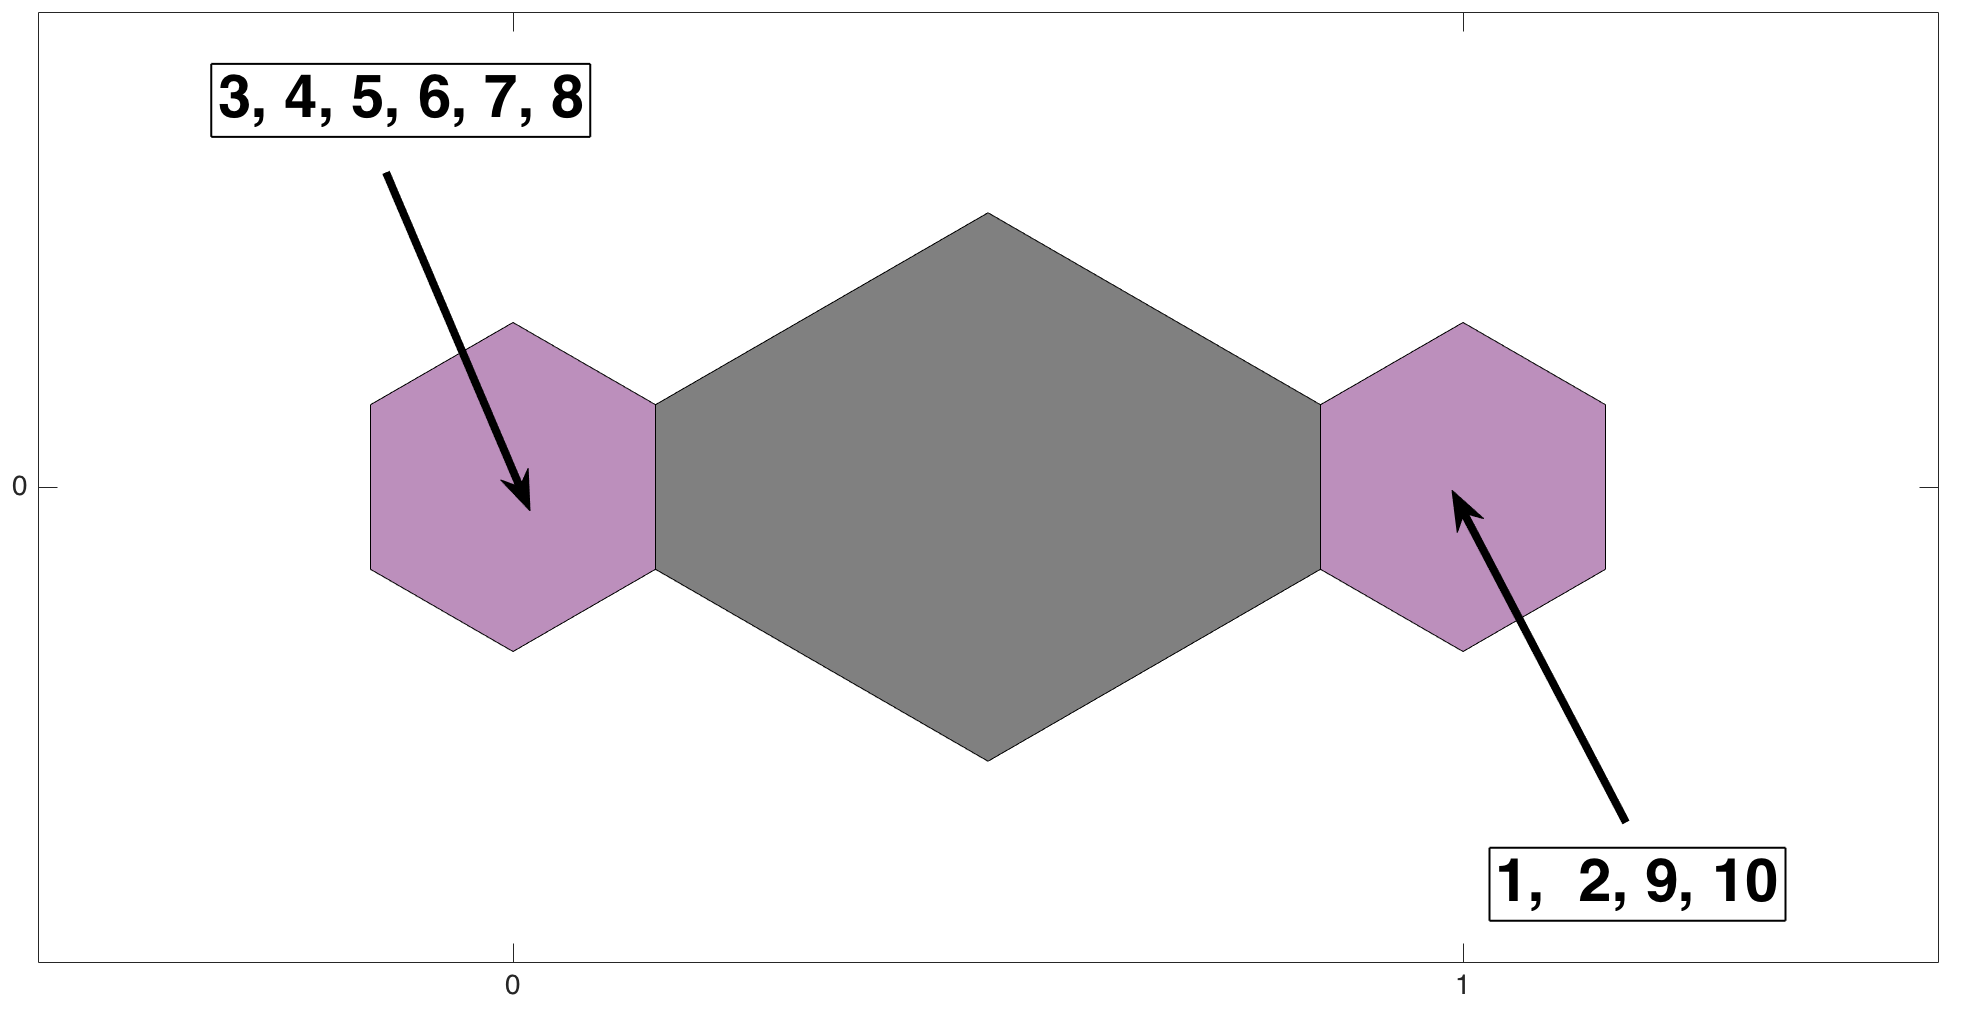
\includegraphics[width=\textwidth]{../image_paper3/images0.01/M31/1D/combine_1D_1by2_all.png}
             }
            \hfill
            \subfloat[$1\times3$~network\label{fig: M31_net_1by3}]{
            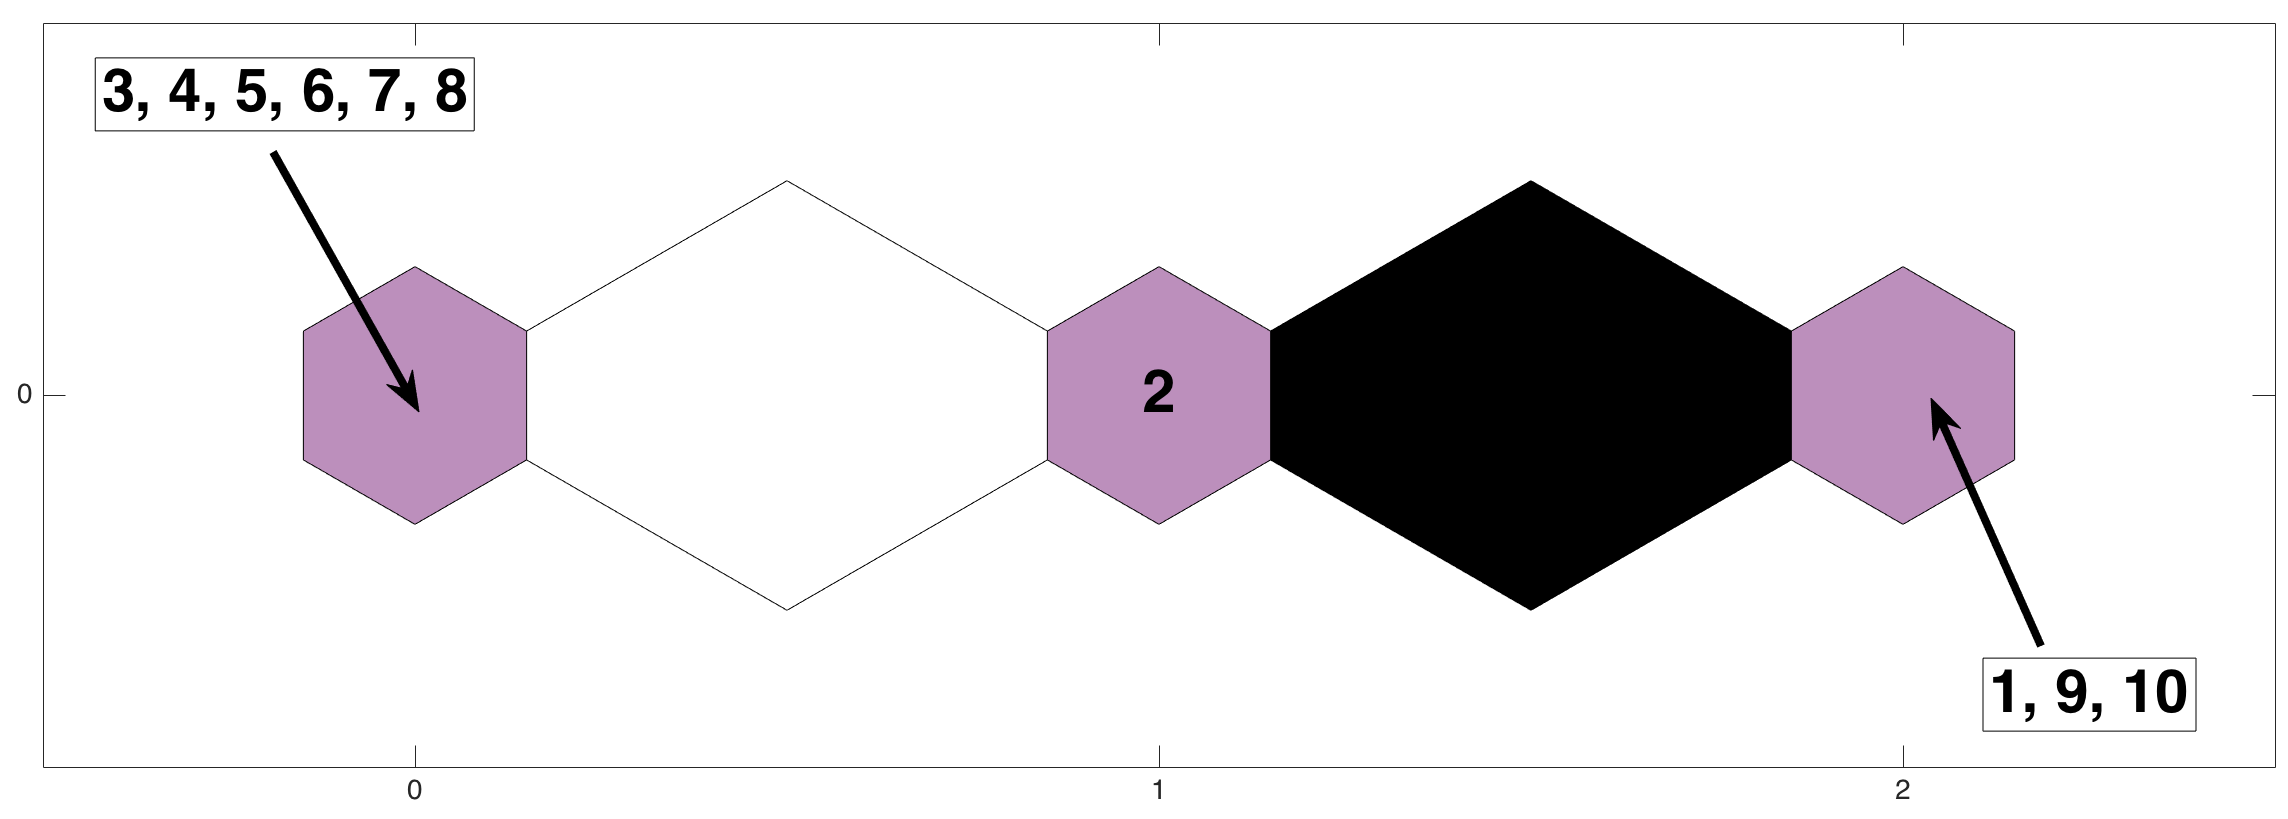
\includegraphics[width=\textwidth]{../image_paper3/images0.01/M31/1D/combine_1D_1by3_all.png}
             }
             \hfill
            \subfloat[$1\times14$~network\label{fig: M31_net_1by14}]{
             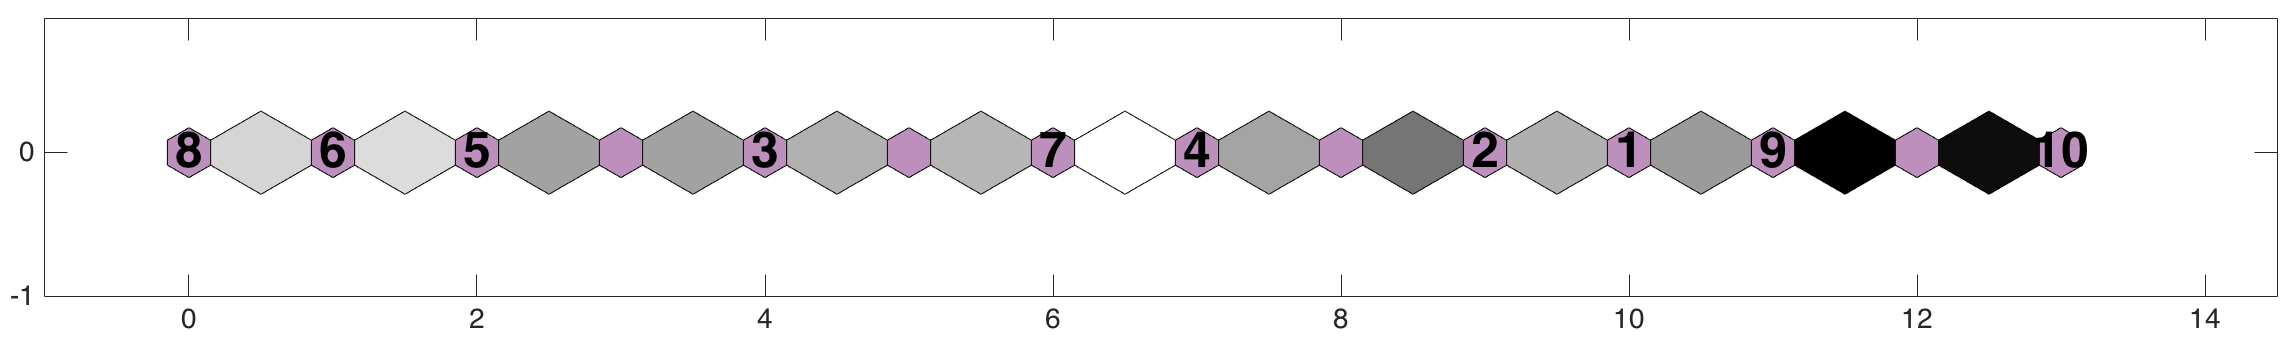
\includegraphics[width=\textwidth]{../image_paper3/images0.01/M31/1D/combine_1D_1by14_all.png}
             }%%% What should I do with this one! It doesn't look good visually
            \caption{SOM of the M31 data from $1\times2$~, $1\times3$~and $1\times14$~grids. The axes show the position of the neurons. The purple Hexagonal shapes represent the neurons. The grey cycle colours show the differences between weight of each neuron with white is the minimum differences and black has the maximum one. The numbers in the plot show the regions that are located in each neuron.}
            \label{fig: M31_nets_1d}
        \end{figure}
        
        %%Network 1by14
        The network with 14 neurons, in Fig.~\ref{fig: M31_net_1by14}, is the first network, that has no neuron to be occupied with more than one region.
        In a higher grid SOM, network pays more attention to smaller details and differences in the input data.
        Therefore, since at least 14 neurons are needed to separate all the 10 regions in M31, we can conclude that some of the regions have very small differences.
        Regions that are located in similar area in M31, like region 7 and 4 (see Fig.~\ref{fig: regions in m31}), are most likely show more similarity to each other.
        In Fig.~\ref{fig: M31_net_1by14}, the most right neuron is occupied by region 10.
        Two black colour between this region and the others indicates the high differences between this neuron and the other ones.
        The region 10 is located in the bulge of M31, and its separation from other regions, which are mostly located around the inner or outer rings, is due to the fact that most of the input values for this region is much higher than the other regions.
        The region 8 occupies the most right neurons in this network, that suggests that this region has the most differences with region 10.
        
        
    \subsection{Inside of the 2 neurons network}%%% I will find better title for this subsection
        %What is going on in this section
        \label{sec: inside_the_2_neurons}
        Using SOMs, we can identify hidden subgroups in our samples. 
        Each of these subgroups were separated from each other, for a reason.
        This reason can vary from having higher values in some specific wavelengths, as discussed in Sec.~\ref{Sec: 1d_cluster}, to some unknown correlations between data, that cannot be seen in other groups or in a Galaxy's data as a whole.
        To investigate the later, we showed the Pearson correlation coefficients for the inputs from regions 3 to 8 in Fig.~\ref{fig: cor_cluster1}, which were clustered together in the $1\times2$ and $1\times3$ networks (see Figs.~\ref{fig: M31_net_1by2} and ~\ref{fig: M31_net_1by3}).
        
        \begin{figure}
        \centering
        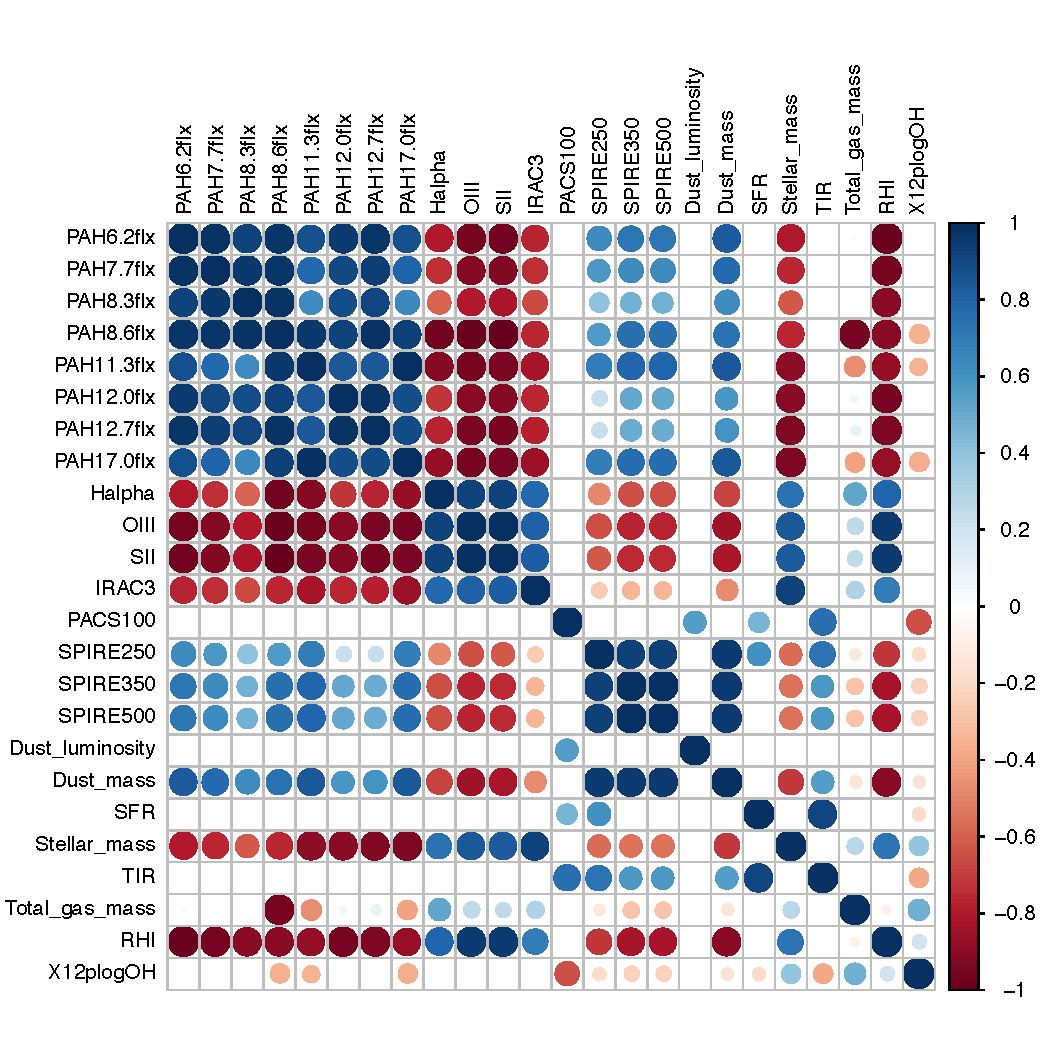
\includegraphics[width=\textwidth]{../image_paper3/images0.01/cor_plots/M31_derived_3_to_8_core_plot_for_paper.pdf}%%% cut the white regions around the figure
        \caption{Same as Fig.~\ref{fig: cor_all}, but here we used data from regions grouped in the left side of the Figs.~\ref{fig: M31_net_1by2} and ~\ref{fig: M31_net_1by3}. }
          \label{fig: cor_cluster1}
        \end{figure}
        
        %%% what regions' version shows and how it compares with the other one:
        In Fig.~\ref{fig: cor_all}, which shows the Pearson correlation coefficients from data in all 10 regions, all the PAHs features highly correlate with each other. 
        Also, there are very strong correlations between all the PAHs features and PACS~100~$\mu$m~, SPIRE 250 to 500~$\mu$m~emission, L$_{\rm dust}$, L$_{\rm TIR}$, SFR, and metallicity.
        However, in Fig.~\ref{fig: cor_cluster1}, 12.0 and 12.7~$\mu$m~PAHs fluxes do not show any significant or strong correlation with PAH fluxes in other wavelengths or most of the other quantities.
        The only exceptions are the strong correlation between PAH flux at 12~$\mu$m and L$_{\rm dust}$, and between 12 and 12.7~$\mu$m PAH fluxes.
        Since there are only 6 regions in this cluster, even one outlier in the data may cause the correlation coefficient become insignificant.
        By removing the outlier, the correlations between 12.0 and 12.7~$\mu$m~PAHs fluxes and the other quantities show themselves. 
        
        For the rest of the PAHs fluxes in Fig.~\ref{fig: cor_cluster1}, there are not any significant correlations with PACS~100~$\mu$m, L$_{\rm dust}$, L$_{\rm TIR}$, SFR, or metallicity, neither.
        They have correlations with SPIRE emission, but they are weaker than the ones with data from all regions.
        Correlations between PAHs features and SFR, and L$_{\rm TIR}$ are well-studied~\citep[e.g.][]{Tielens08,Peeters04}. 
        Many groups used PAHs features as a tracer of SFR by finding correlations between 
        PAHs emission and SFR derived from extinction corrected \halpha~\citep[e.g.][]{Shipley16,Khramtsova13,Calzetti07}.
        These correlations are seen in Fig.~\ref{fig: cor_all}, when we considered the data from all regions, but not in Fig.~\ref{fig: cor_cluster1} when considering the clustered data.
        Further analyses show that the absence of correlations between PAHs features and SFR, is because of one outlier in data. 
        When we disregard the outlier data, high correlations between 6.2 to 11.3~$\mu$m~PAHs features and SFR (and L$_{\rm TIR}$) reappear.
        Strong ant-correlation between 6.2 to 11.3~$\mu$m~PAHs features and RHI, stellar mass, \halpha, \sii, \oiii, and IRAC~5.6~$\mu$m~emission in Fig.~\ref{fig: cor_cluster1} had not be seen in Fig.~\ref{fig: cor_all}.
     %   In Fig.~\ref{fig: cor_cluster1}, 6.2, 7.7, 8.3, 8.6, and 11.3~$\mu$m~PAHs features show strong anti-correlations with RHI, stellar mass, \halpha, \sii, \oiii, and IRAC~5.6~$\mu$m~emission.
     
        Anti-correlations between PAHs features and the \halpha, \sii, and \oiii~emission could be the result of one the followings. 
        First, the optical data are not corrected for dust extinction.
        The PAHs features correlate with dust, and \halpha emission is sensitive to dust extinction.
        Therefore, more PAHs features, means more dust and less \halpha~emission (The same for \sii~and \oiii~emission).
        Second, it is the effect of observing apertures.
        If the regions are located in the edge of the H {\sc II} regions we would expect too see more PAHs and less \halpha~emission. %%% reference?
        The anti-correlations between 6.2 to 11.3~$\mu$m~PAHs features and RHI have been seen in other studies, too~\citep[e.g.][]{Dim15, Gordon08, Wu06}.
        \cite{Wu06} discussed these ant-correlations could be the result of destruction of the PAHs due to the high amount of the harder radiation (thus higher RHI).
        On the other hand, \cite{Gordon08} argued that the harder radiation could make the photodissociation regions (PDRs) smaller.
        The PAHs features are mostly coming from the PDRs that are surrounded by H {\sc II} regions, and the PAHs features underlying continuum emission is from the H {\sc II} regions.
        Therefore, the lower flux of the PAHs features could be the result of the smaller size of PDRs.
        The later reason, which could also describe the anti-correlation between PAHs features and \halpha~emission, seems to be the more probable one. 
        %%% The anti correlation with stellar mass?!! with IRAC3?!!
        
       Despite the fact that some of the (anti)-correlations in Fig.~\ref{fig: cor_cluster1} might have physical meanings, we have to mention that, we only used 6 regions to calculate these correlation coefficients.
       Having 6 data points as a sample of the study is not high enough to have a strong conclusion about the PAHs in M31.%%% it doesn't sound right:((
        However, we can conclude that since the correlation coefficients derived from the clustered data (Fig.~\ref{fig: cor_cluster1}) differs from correlation coefficients derived from the data from the all regions (Fig.~\ref{fig: cor_all}), SOM separated a hidden cluster of the data, which their properties are different than the others. %%Again eh!
        
        
        
        
        

 %----------------------------------------------------------------------------------------
%----------------------------------------------------------------------------------------
%----------------------------------------------------------------------------------------
%Result Part 2: 2D SOMs
%----------------------------------------------------------------------------------------
%----------------------------------------------------------------------------------------
%----------------------------------------------------------------------------------------
 \section{Two dimensional self-organizing maps}
 \label{sec: 2d_cluster}
    Although 1D networks are great to have a general idea about the data, neurons in 1D maps have maximum two neighbours, which causes some limitation in the results.
    In 2D networks, each neuron has two to six neighbours, which allowed them to to capture a whole picture of the complicated relations in the input data.
    Therefore, we created $10\times10$ 2D networks to study the data in details.
    As mentioned in previous sections, the size of SOMs are arbitrary and users must decide about it based on what their goals of using SOMs are.
    In this section we chose $10\times10$ size despite that we knew, from the size of our input data, that most of the neurons would be empty.
    Using 2D networks, we are mostly interested in the ability of the SOMs in showing underlying structure of the data rather than its clustering features.
    \import{../image_paper3/text_files/image_texts/}{all.tex}
    Fig.~\ref{fig: all_derived_ones} shows the 2D SOM of M31 data.
    Similar to the Fig.~\ref{fig: M31_net_1by14}, all the 10 regions completely separated from each other in Fig.~\ref{fig: all_derived_ones}.
    
    Regions 4 and 7 are in the top left of Fig.~\ref{fig: all_derived_ones} with very bright colour between their neurons, which presents that these two regions are very similar.
    Considering the position of these two regions in M31 (Both of these regions are right on the edge of the star forming rings in the galaxy), similarity of these two regions were predictable.
    Position of region 3 on the SOM is close to the position of regions 4 and 7, but with darker colour between the nodes. 
    In Fig.~\ref{fig: regions in m31} it is clear that, this region in M31 is closer to regions 4 and 7 than any other region, but it is on the outer side of the star forming ring.
    Regions 5 and 6 are in their second neighbourhood on the SOM, with a medium gray colour between them.
    These two regions are around the inner ring of the galaxy.
    Regions 8 and 6 are both in the inner ring of M31, but region 6 is in the region with more star forming activities, which could be the main reason for their relative distance in the SOM in Fig.~\ref{fig: all_derived_ones}. 
    
    Regions 1 and 9 are close to each other, and in the same side of the star forming ring. 
    However, region 1 is in an area of the galaxy with lesser diffuse \halpha~emission than region 9, that might be the reason for their distances in SOM.
    Region 2 is more distant from other regions in the galaxy, and placed in the star forming ring.
    However, similar to regions 1 and 4, region 2 is located in an area of the galaxy with less diffused \halpha~emission.
    Therefore, place of region 2 in the SOM is more favoured towards regions 1 and 4. 
    Region 10 is placed in the bulge of the galaxy, and its position on the SOM is isolated from all the other regions by a strip of a dark colours. 
    
    In order to analyse effects of any input data on the final SOM, in the following we created SOMs from various subsets of data.
    We compare results of the subsets with one another and with SOM created from all data in Fig.~\ref{fig: all_derived_ones}.

    \subsection{Subsets}
    \label{sec: subsets}
            For analysing subsets, we creating SOMs by using only PAHs data, as well as using all data except PAHs ones (Fig.~\ref{fig: PAHS_or_not_PAHs}).
             \import{../image_paper3/text_files/image_texts/}{PAHS_or_not_PAHs.tex}
            Comparing the SOM from all data in Fig.~\ref{fig: all_derived_ones} with the SOMs in Fig.~\ref{fig: PAHS_or_not_PAHs}, showed that the general position of regions in those networks are the same. 
            The region 10 is in one corner of the all three networks.
            However, in Fig.~\ref{fig: all_derived_ones} and Fig.~\ref{fig: wt_pahs}, region 10 is isolated from the other regions, while in Fig.~\ref{fig: only_pahs}, region 10 is much less isolated and only shows complete dissimilarity with region 8.
            Regions 9 and 10 are totally isolated in SOMs in Fig.~\ref{fig: wt_pahs}, but in Fig.~\ref{fig: only_pahs}, they are more similar to other regions.
            In both SOMs in Fig.~\ref{fig: PAHS_or_not_PAHs}, there are dissimilarities between regions in M31 but in Fig.~\ref{fig: wt_pahs}, the colours are much darker than the ones in Fig.~\ref{fig: only_pahs}.
            This indicates that there are more similarity between PAHs features from all 10 regions then the other input data.
            
            We increased the dimension of input data in Fig.~\ref{fig: only_pahs} (PAH only data), gradually, by adding data from other quantities of galaxies to the input data. 
            The order of adding data is the same as order of data in Fig.~\ref{fig: cor_all}, i.e. SOM in Fig~\ref{fig: inc_D_col3s}a was created from PAHs data and H$\alpha$ emission as input data, SOM in Fig~\ref{fig: inc_D_col3s}b created from PAHs, H$\alpha$ emission and [\sii] continuum as input data, and so on. 
            \import{../image_paper3/text_files/image_texts/}{col3byall.tex}
            
            SOM algorithm assigns random weight to each network, that causes the overall position of regions in networks (even with the same input data) changes in each run of the algorithm.
            However, the position of each region regarding to other regions changes dramatically only because of the new sets of input data is given to the algorithm (assuming all the initial values for the run are intact).
            In all SOMs in Fig~\ref{fig: inc_D_col3s}, region 10 is located in the corner of the SOMs, but in  Figs~\ref{fig: inc_D_col3s}a,~\ref{fig: inc_D_col3s}d,~\ref{fig: inc_D_col3s}g,~\ref{fig: inc_D_col3s}k, and ~\ref{fig: inc_D_col3s}l, it is placed in the left side of the SOMs and in the others it is in the right side of the networks.
            In our discussion on differences between networks, we do not address the changes in the network due to initialization of the SOM algorithm and only consider the effect of changing the input data in the network.
            
            Comparing Figs.~\ref{fig: inc_D_col3s}a to ~\ref{fig: inc_D_col3s}o shows that adding \halpha~emission data to PAHs features causes regions 9 and 10 become isolated. 
            Increasing dimension of the input data makes region 10 more isolated.
            The relative position of regions 4 and 7 stays the same with increasing the input data. 
            Adding SPIRE 350, 500~$\mu$m emission and L$_{\rm dust}$ do not have any adequate effect on the networks.
            Stellar mass, total gas mass, dust mass and RHI data alternate the distances between neurons effectively, but it seems that adding SFR, L$_{\rm TIR}$ and metallicity data revoke those changes.
            
            We generated other subsets of the data based on the results in Figs~\ref{fig: inc_D_col3s} to study effects of the input data on SOMs, further.
            Subset 1, that are listed in Tab.~\ref{tab: subset1}, includes all the inputs data except data from stellar mass.
            Tab.~\ref{tab: subset5} is the list of data that were used in a subset 2, which includes all data except the fact that instead of the individual PAH fluxes we added them all together and have total PAH flux. 
            For subset 3 ( in Tab.~\ref{tab: subset6}), we removed SPIRE 250 and 500~$\mu$m from subset 2.
            Figs.~\ref{fig: subset1} --~\ref{fig: subset6} show SOMs that are created by data from subsets 1 to 3, respectively.
            The rest of the subsets are discussed in the Appendix.~\ref{sec: app_2d_soms_SOMN}.

            The results from Table~\ref{tab: subset1} is shown in Fig.~\ref{fig: subset1}. 
            In this SOM compare with the SOM from all the data in Fig.~\ref{fig: all_derived_ones}, regions 1 and 9 are closer to region 10. 
            Regions 1 and 9 are the ones with lowest stellar mass values, and region 10 has the highest stellar mass value among those 10 regions. 
            Since the differences in the amount of the stellar mass were one of the most distinct differences between these three regions, removing stellar mass from input data reduced the distance between these regions.
            Regions 5, 6 and 8 are in the same relative distance from each other as in Fig.~\ref{fig: all_derived_ones}, but they all are closer to the position of the region 10.
            Distance between regions 2 and 3 is reduced but in the meantime the colour between them became darker.

            \import{../image_paper3/text_files/tables/}{subset1.tex}
            \import{../image_paper3/text_files/image_texts/}{subset1.tex}

            Changing from separate values for each PAH features to a single value for the total PAHs caused small changes to the SOM map in Fig.~\ref{fig: subset5} compare to the one in Fig.~\ref{fig: all_derived_ones}. 
            Distance between the relative position of regions 6 and 8 increased significantly, while the position of region 2 moved closer to the positions of regions 4 and 7.
            The winner neurons for regions 3 and 5 moved towards each other, but the colours between them became much more darker. 

            \import{../image_paper3/text_files/tables/}{subset5.tex}
            \import{../image_paper3/text_files/image_texts/}{subset5.tex}

            Fig.~\ref{fig: subset6} shows the SOM generated from data that are listed in Tab.~\ref{tab: subset6}, which includes all the data from Tab.~\ref{tab: subset5} except SPIRE 250 and 500~$\mu$m emission.
            Although for most of the regions we see the changes in their positions, the colours between neurons changed, too. 
            %Therefore, we can conclude that these changes caused by the differences in the initial assigned weights.
            The distance between the positions of the regions 4 and 2 are increased.
            The same happened for distances between regions 7, 3 and 6.
            In both cases, SPIRE 250 and 500~$\mu$m emission of these regions are similar to one another, and removing these two parameters from input data moved the positions of the regions further from each other. 
            \import{../image_paper3/text_files/tables/}{subset6.tex}
            \import{../image_paper3/text_files/image_texts/}{subset6.tex}
            
            %Subsets, that some of them  are studied in this section, can be used to learn about the effect of each input on the map as well as they can be used to predict unobserved quantities in the galaxy.
            \subsubsection{Prediction observing data using M31}
        
                On SOMs we can see relations between the input data from each region regarding to the other regions.
                These relations are shown by colour in SOMs, when white is 100 per cent similarity and black is 0 per cent similarity.
                Therefore, we have the probability distribution of quantities of each values given data from other regions.
                We can use these probability distribution to estimate missing data for regions. 
                
                To demonstrate this conclusion, we assumed the stellar mass value for region 1 is unknown.
                Therefore, we need a SOM that are generated from all the inputs data for all regions except stellar mass (e.g subset 1 in Fig.~\ref{fig: subset1}).
                \import{../image_paper3/text_files/image_texts/}{sim_subset1.tex}
                We found the shortest path between region 1 and the other regions and measure their relative similarity ($p_j$).
                Assuming the maximum similarity is 100 per cent between two neurons (white colour), we multiply the similarity values along the shortest path between two regions to find $p_j$ between region 1 and the other regions (Fig.~\ref{fig: sim_subset1}).
                In both Figs.~\ref{fig: subset1} and ~\ref{fig: sim_subset1} are clear that region 1 shows more similarity to regions 2 and 9 than the others and the most dissimilarity to region 8. 
                
                We measured probability of stellar mass given other quantities of the region 1 ($P(m_1\mid \forall_1)$) using Equation~\ref{equ: prob1}.
                \begin{equation}
                \label{equ: prob1}
                    P(m_1\mid \forall_1) = \sum_{j=2}^{10}p_j*m_j
                \end{equation}
                Where $m_1$ is the stellar mass of region 1 and $m_j$ is the stellar mass of region j (any other region).
                We estimated the stellar mass to be $\sim1377$~M$\odot$ which is 10 per cent less than the observed values.
                This type of the prediction from SOM networks can be used to predict observation values in observational proposals or can be used in pre-phase studies of the big missions such as the James Webb Space Telescope (JWST) and LLST.
                

    \subsection{Validating networks using M101 data}
    Another application of SOM for nearby galaxies is that to apply the trained networks on the data from other galaxies in order to prediction properties of the regions in them. %%eh
    As an example of this application, we generated an SOM using data from M31 that held in common with M101 data (Fig.~\ref{fig: subset9}a). 
    In this SOM, the same as the others, region 10 is separated from other regions in M31.
    Regions 7 and 4 are close to each other with very light colours between their neurons, and the same as the other SOMs regions 6, 8, and 5 are close to each other, but with medium dark colour between them.
    \import{../image_paper3/text_files/image_texts/}{subset9.tex}
    
    We applied the SOM created using M31 data in Fig.~\ref{fig: subset9}a on M101 data (Fig.~\ref{fig: subset9}b).
    Region 6 in M31 and region 2 in M101 both occupied the same neuron in the network in Fig.~\ref{fig: subset9}, which immediately suggest that these two regions have similar properties. 
    Region 2 in M101 is a bright H {\sc II} region that is located at the end of the one of the M101 spiral arm (see Fig.~\ref{fig: regions in m101}). 
    Region 6 in M31 is located near the inner ring of the galaxy (see Fig.~\ref{fig: regions in m31}).
    Both regions have relatively low amount of PAHs emission and medium amount of the SFR regarding the other regions in the galaxy, which makes them very similar regions.
    
    Region 7 in M101 is located in the nucleus of the galaxy and have relatively higher quantities than the other regions.
    This region is located in the top right side of the network in Fig.~\ref{fig: subset9}, which is close to location of region 10 in the network.
    Since the bulge of a spiral galaxy has different environment from its nucleus, region 7 in M101 and region 10 in M31 are not occupied the same neuron in the SOM, and have a medium grey colour between their neurons.

    Region 1 in M101 is located near the nucleus of M101 (see Fig.~\ref{fig: regions in m101}), but has considerably lower values in all the quantities than the ones in region 7.
    The lower values for fluxes of the PAH features, and relatively moderate amount of the SFR caused this region places between region 4 and 5 of M31 in the network. 
    Fig.~\ref{fig: subset9}b shows that region 4 in M101 is separated itself from other regions and located between region 9 and 10 in M31.
    \cite{Gordon08} showed that this region is a diffuse nebula in M101, with high amount of fluxes of PAH features. 
    This region also shows a high amount of the SFR and the stellar mass, which describes why the location of region 4 from M101 in the SOM is close to regions 9 and 10 from M31.
    
    In this section we showed that we can use networks that are created by data from nearby galaxies, to study the properties of other galaxies in a fast way.
    We should note that we created our networks using values for 26 quantities from 10 regions in M31, which does not consider as a "big sample".
    Increasing dimension of the data and the number of regions would help to have more reliable networks.
    
    

%----------------------------------------------------------------------------------------
%----------------------------------------------------------------------------------------
%----------------------------------------------------------------------------------------
%Summery
%----------------------------------------------------------------------------------------
%----------------------------------------------------------------------------------------
%----------------------------------------------------------------------------------------
\section{SUMMARY}
\label{sec: summary}
Self-organizing maps can be used to explore hidden subgroups and underlying structure of the data.
In this project we investigated applications of the Self-organizing maps in data from nearby galaxies.
We utilized the SOM method to study data from two well-studied galaxies; M31 and M101.
Data from nearby galaxies can be clustered in various networks with different sizes/dimensions based on the information needed from the data. 
A network with one dimension and a few neurons, can be used for general classification, while for more detailed clustering, a higher number of neurons should be used.

Using smaller-sized self-organizing maps, the M31 data were clustered in 2 major groups; we found correlations that could not have otherwise been seen without clustering.
For example in Sec.~\ref{sec: inside_the_2_neurons}, we found that six of the regions in M31 create a subgroup of data, that have lower amount of PAHs flux.
Flux from the PAHs features in these regions highly anti-correlated with \halpha~emission despite that considering Flux from the PAHs features in all regions highly correlates with SFR.
Our analyses of smaller-sized networks showed that using this method we can find hidden subgroups in data to extend our knowledge of inside the galaxies.

In the maps with larger sizes, networks can be used to illustrate the relative relations of the regions with one another.
We found the relative similarity between M31 regions, by varying the size of networks.
A one-dimensional network with 14 neurons was needed in order to
separate all 10 regions; we concluded that some of the region in M31 (e.g. regions 4 and 7) are very similar.
A two-dimensional networks provide us a more complete picture of the data.
Using these networks, we show a relative relations between regions in M31.

We introduced self-organizing maps as a method that can be used to predict the amount of various quantities based on the relative positions of the regions in the networks.
By converting the relative distance between regions to the probability distribution function, we could predict unobserved/unmeasured properties of the galaxies with 10 per cent uncertainty.
We also applied the SOMs from M31 data to M101 data and found regions with similar properties in both galaxies placed in close regions in the SOMs.
We show that using this ability of the SOM, we can predict properties of regions in other nearby galaxies very fast.

 
%----------------------------------------------------------------------------------------
%----------------------------------------------------------------------------------------
%----------------------------------------------------------------------------------------
%biblio
%----------------------------------------------------------------------------------------
%----------------------------------------------------------------------------------------
%------------------

\addcontentsline{toc}{section}{Bibliography}
\bibliographystyle{apj.bst}
\bibliography{ref_paper3.bib}